

\section{The algorithm}


    \begin{frame}{The problem}
        Genome and protein alignment are fundamental bio-informatics techniques used to compare sequences of DNA, RNA, or proteins to identify regions of similarity.

        \vspace{10pt}
        
        These alignments reveal evolutionary relationships, functional similarities, or conserved regions across species or within different genes and proteins of the same organism.
    \end{frame}

    

    \begin{frame}{The challenge}
        Genomes can consist of billions of base pairs (the human genome has over 3 billion base pairs!).
        
        Aligning such large datasets requires significant computational resources.

        \vspace{10pt}

    \begin{minipage}{0.49\linewidth}
        \begin{figure}
                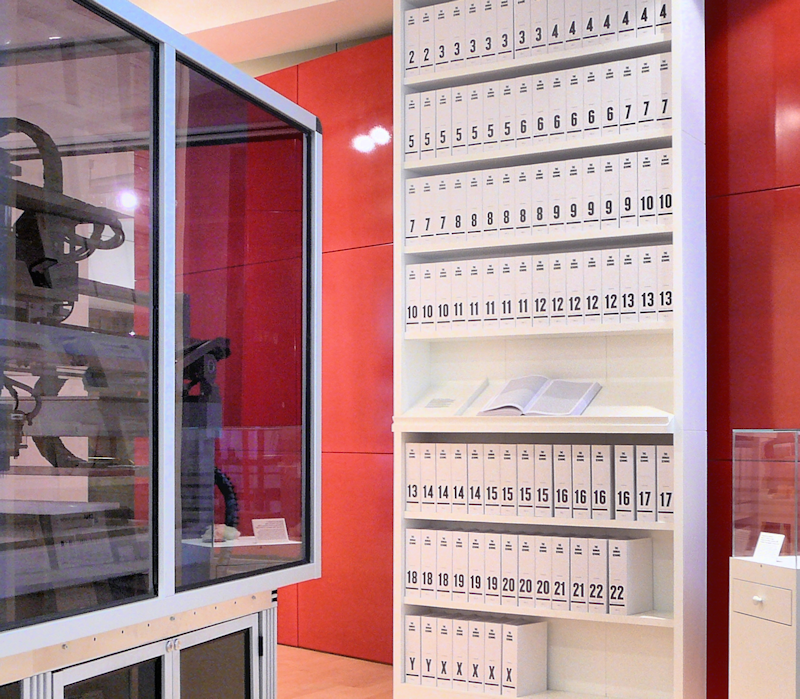
\includegraphics[width=0.8\linewidth]{human_genome_printout.png}
                \caption{Human genome printout}
            \end{figure}
    \end{minipage}
    \begin{minipage}{0.49\linewidth}
        \begin{figure}
            
\includegraphics[width=1\linewidth]{human_genome_book.JPG}
            \caption{Enter Caption}
        \end{figure}
    \end{minipage}
    \end{frame}





    \begin{frame}{How does the algorithm work?}

        The Smith-Waterman algorithm is a dynamic programming algorithm used specifically for local sequence alignment, that is to identify the most similar subsequences between two sequences.

        \vspace{20pt}

        \begin{figure}
            \centering
            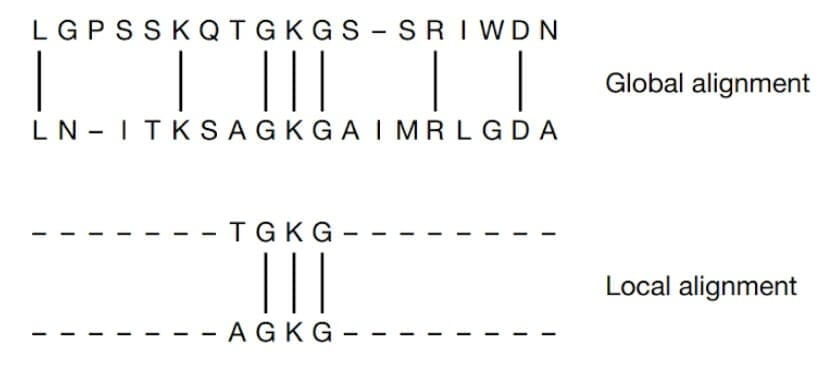
\includegraphics[width=0.5\linewidth]{global_vs_local_alignment.jpg}
        \end{figure}

    \end{frame}



    \begin{frame}{How does the algorithm work?}

        A scoring matrix $H$ is created and filled as follows. The first row and column are initialized to zero.
        \[
            H(i, j) = \max \begin{cases} 
            0 \\
            H(i-1, j-1) + s(i, j) & \text{(match/mismatch)} \\
            H(i-1, j) + g & \text{(deletion)} \\
            H(i, j-1) + g & \text{(insertion)} \\
            \end{cases}
        \]

        \begin{itemize}
            \item $H(i, j)$ is the score at position $(i, j)$,
            \item $s(i, j)$ is the score for a match or mismatch,
            \item $g$ is the penalty for a gap. It can be a function of the gap size. 
        \end{itemize}
        
    \end{frame}

     \begin{frame}{Algorithm data dependencies}

        \begin{minipage}{0.49\linewidth}
            Highlight the dependence of $H(i, j)$ from:
        \begin{itemize}
            \item the previous element along the diagonal $H(i-1, j-1)$,
            \item the previous element along the column $H(i, j-1)$,
            \item the previous element along the row $H(i-1, j)$.
        \end{itemize}

        \vspace{10pt}

        Furthermore, sequences can be insanely huge!
        \end{minipage}
        \begin{minipage}{0.49\linewidth}
            \begin{figure}
            \centering
            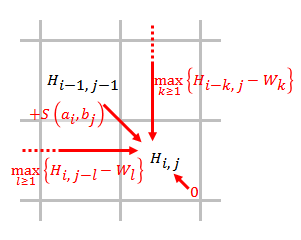
\includegraphics[width=1\linewidth]{algorithm_image.png}
        \end{figure}
        \end{minipage}
        

        

    \end{frame}